\documentclass{beamer}
%\usetheme{Ilmenau}
%\usecolortheme{beaver}

\usepackage[slovak,american]{babel}
\usepackage[utf8]{inputenc}
\usepackage{graphicx}
\usepackage{adjustbox}
 \usepackage{xcolor}
 
 \newsavebox\MBox
\newcommand\Cline[2][red]{{\sbox\MBox{$#2$}%
  \rlap{\usebox\MBox}\color{#1}\rule[-2.2\dp\MBox]{\wd\MBox}{1pt}}}

%\usefonttheme{serif}

%\definecolor{UKOrange}{HTML}{ef9424} %
\definecolor{UKOrange}{HTML}{7a2c18} %
\definecolor{UKBrown}{HTML}{a96d5e} %
\definecolor{UKLight}{HTML}{d8b6ab} %
\definecolor{UKDark}{HTML}{7a4f44}
\definecolor{UKDarker}{HTML}{4d312b} 
\definecolor{UKDarkest}{HTML}{2e1e1a}
\definecolor{UKRed}{HTML}{bf1f1c}

\setbeamertemplate{footline}[frame number]{}
\setbeamertemplate{navigation symbols}{}

%\usecolortheme{beaver}
\setbeamertemplate{itemize item}[square]
\setbeamercolor{itemize item}{fg = UKBrown}
\setbeamercolor{itemize subitem}{fg = UKLight}
\setbeamercolor{enumerate item}{fg = UKDark}

\setbeamercolor{footnote}{fg=UKLight}
\setbeamercolor{footnote mark}{fg=UKLight}
\setbeamerfont{footnote}{size=\tiny}
\renewcommand\footnoterule{}

\usetheme{default}
\beamertemplatenavigationsymbolsempty
\setbeamercolor{title}{fg=white, bg=UKBrown}
\setbeamercolor{frametitle}{fg=white, bg=UKBrown}
\setbeamercolor{block title}{bg=UKBrown, fg= white}
\setbeamercolor{block body}{bg =UKLight, fg = UKDarkest}

\setbeamercolor{block title alerted}{bg=UKOrange, fg= white}
\setbeamercolor{block body alerted}{bg =UKLight, fg = UKDarkest}


%\setbeamercolor{section in toc}{fg = UKBrown}
%\setbeamercolor{section in toc}{fg = UKDarkest}

% odstrani gulicky
\renewcommand*{\slideentry}[6]{}

\useoutertheme[subsection=false]{miniframes}
\AtBeginSection[]{\subsection{}}

\setbeamercolor{below lower separation line head}{bg=UKDark}
\addtobeamertemplate{headline}{}{%
  \begin{beamercolorbox}[colsep=0.5pt]{below lower separation line head}
  \end{beamercolorbox}
}
%\setbeamercolor*{mini frame}{fg=white,bg=UKRosy}
\setbeamercolor{section in head/foot}{fg=UKLight, bg=UKDark}

\usepackage{etoolbox}
\makeatletter
\preto{\@verbatim}{\topsep=0pt \partopsep=0pt }
\makeatother

%\setbeamertemplate{itemize/enumerate body begin}{\normalsize}
%\setbeamertemplate{itemize/enumerate subbody begin}{\normalsize}




%\newcommand{\codeblock}[2]{ \begin{block}{#1} \begin{verbatim}#2\end{verbatim}\end{block}}

%\defbeamertemplate*{title page}{customized}[1][]
%{
%  \begin{centering}
%    \begin{beamercolorbox}[sep=8pt,center]{title}
%      \usebeamerfont{title}\inserttitle
%    \end{beamercolorbox}
%  \end{centering}
%  \bigskip
%
%\begin{columns}[onlytextwidth,T]
%
%
%  \column{27mm}
%  \includegraphics[width=27mm]{images/logoFMFI.png}
%  
%  \column{\dimexpr\linewidth-54mm-6mm}
%  \centering
%  \vspace{5mm}  
%  \usebeamerfont{author}\insertauthor\par
%  \vspace{5mm}
%  \usebeamerfont{institute}\insertinstitute\par
%
%  \column{27mm}
%  \includegraphics[width=27mm]{images/logoUK.png}  
%\end{columns}
%\centering
%\vspace{7mm}
%  \usebeamerfont{date}\insertdate\par
%}

\DeclareMathOperator*{\argmin}{arg\,min}
\newcommand{\e}[1]{$\cdot 10^{#1}$}

%\newcommand{\codeblock}[2]{ \begin{block}{#1} \begin{verbatim}#2\end{verbatim}\end{block}}



\title[3. cvičenie]{Advanced Image Processing - Color Spaces}
\author[Kocur]{Ing. Viktor Kocur \\{\small viktor.kocur@fmph.uniba.sk}}
\institute{DAI FMFI UK}
\date{9.10.2019}

\begin{document}
\selectlanguage{slovak}

\begin{frame}
  \titlepage
\end{frame}

%\begin{frame}
%  \tableofcontents
%\end{frame}

\section{Colors}
\subsection{HSV}
\begin{frame}
\frametitle{HSV}
  \begin{block}{HSV}
  HSV is a color model aimed at intuitive use (user-friendly model). Hue determines the position on a color ring, S stands for saturation and V for value, which determines the intensity,
  
  \end{block} 
  
  \begin{block}{rgb2hsv}
  rgb2hsv(I) - returns image I in HSV format.
  \end{block} 
  
    \begin{block}{hsv2rgb}
  hsv2rgb(I\_hsv) - does the same but other way around.
  \end{block} 
\end{frame}

\begin{frame}
\frametitle{HSV - Exercise}
  \begin{block}{HSV}
  Use the GUI from last week, but instead of RGB sliders use HSV. When displaying the image you have to convert it to RGB before displaying.
  \end{block} 

\end{frame}

\subsection{CIE Lab}
\begin{frame}
\frametitle{CIE Lab}
  \begin{block}{CIE Lab}  
  CIE L* a* b* is a three element model. L stands for luminance, a is position on the green-red axis and b is position on the blue-yellow axis.
  \end{block} 

  
  \begin{block}{rgb2lab}
  rgb2lab(I) - returns the image I in the Lab format
  \end{block} 
  
    
  \begin{block}{lab2rgb}
  lab2rgb(I\_lab) - the same but in reverse
  \end{block} 

  
  \begin{block}{Exercise}
  Change the GUI so the sliders represent the Lab color space.
  \end{block} 
\end{frame}

\subsection{CMY a CMYK}

\begin{frame}
\frametitle{RGB}
  \begin{block}{RGB}
  RGB is an additive model. The colors are added to a black background.
  \end{block} 

  \begin{center}
  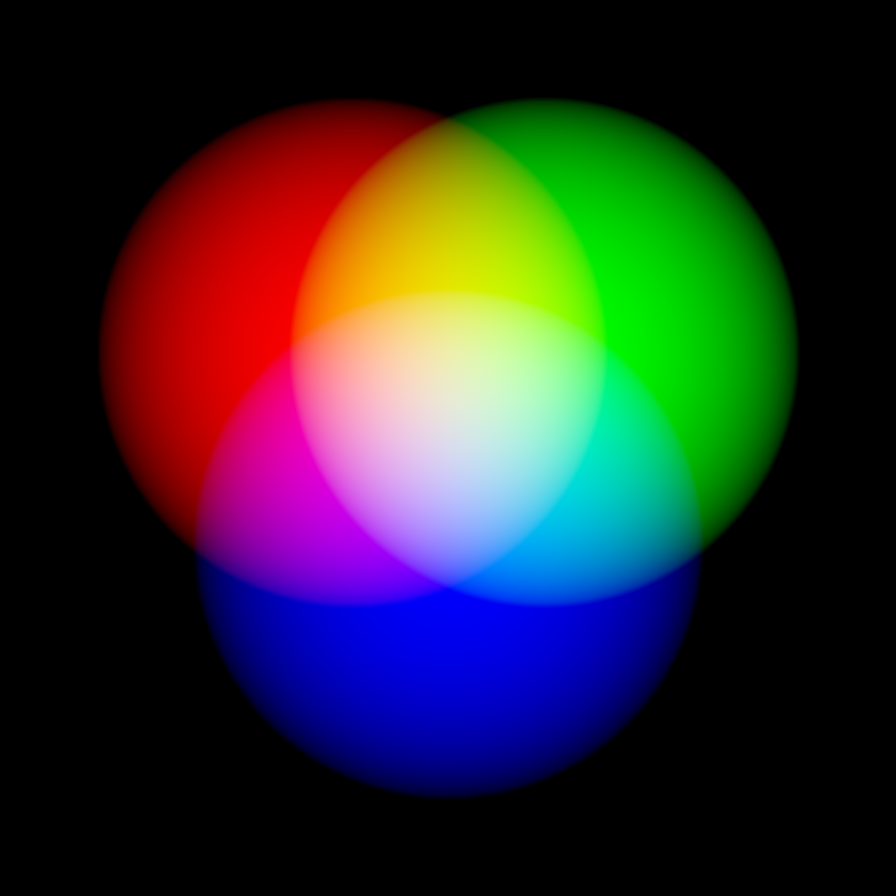
\includegraphics[height=0.5\textheight]{RGB.png}
  \end{center}
\end{frame}

\begin{frame}
\frametitle{CMY}
  \begin{block}{CMY}
  CMY is subtractive model, e.g. we add colors on a white background. If we add all of the colors we will get the black color.
  \end{block} 

  \begin{block}{CMYK}
  CMYK also has a black component which is useful for printing applications.
  \end{block} 

  \begin{center}
  
\includegraphics[height=0.5\textheight]{CMY.png}
  \end{center}
\end{frame}

\begin{frame}
\frametitle{CMY vs. RGB}
  \begin{block}{CMY}
  Conversion from RGB to CMY C~=~255~-~R, M~=~255~-~G a Y~=~255~-~B
  \end{block} 
  
  \pause

  \begin{block}{RGB}
  In reverse: R = M + Y, G = C + Y, B = C + M
  \end{block} 
\end{frame}

\begin{frame}
\frametitle{Euclidian distance}
  \begin{block}{Exercise}
  Write a scipt which displays the image farby.png and using the function ginput lets user pick three points in the image. Compare the distances of colors for the pairs of points in the RGB, HSV and Lab color spaces. Distance in the Lab spectrum should be the most representative of what humans perceive as similar colors.
  \end{block} 
  
    \begin{block}{Euclidian distance}
  \begin{equation*}
  \rho_e(\vec{a}, \vec{b}) = \sqrt{\sum_{i=1}^n (a_i - b_i)^2}
  \end{equation*}
  \end{block} 

  \begin{block}{ginput}
  [x ,y] = ginput(n) - returns vector x and y with coordinates of n points which are captured in the active figure by user
  \end{block} 
\end{frame}


\section{Indexed images and pseudocolors}
\subsection{Pseudocolors}
\begin{frame}[fragile]
\frametitle{Pseudocolors}
  \begin{block}{Pseudocolors}
  We can use pesudocolors to color a grayscale image.
  \end{block} 
  
  \begin{block}{colormap}
  colormap(map) - changes the map with which the image is drawn. Map can be preset (jet, hsv, copper, winter, gray, bones), or any matrix of shape  $n \times 3$ where each row represents an RGB color triple.
  \end{block} 

  \begin{block}{Code}
  \begin{verbatim}
  BW = imread('medical.pgm');
  imagesc(BW);
  colormap(hsv);\end{verbatim}
  \end{block} 
\end{frame}

\subsection{Indexed images}
\begin{frame}[fragile]
\frametitle{Indexed images}
  \begin{block}{Indexed image}
  Indexed image is an image where each pixel is not represented by an RGB triple, but with a specific image. To draw the image it is necessary to have a map which connects the index with a color. The map is a matrix of of shape  $n \times 3$ where each of the n rows represents an RGB color triple.

  \end{block} 
\end{frame}

\begin{frame}[fragile]

  \begin{block}{rgb2ind}
  [X, map] = rgb2ind(I,n) - returns indexed image X with n colors and a map with shape $n \times 3$. \\
    X = rgb2ind(I,map) - returns indexed image X for a given image I and a map.
  \end{block}   
  
  
    \begin{block}{imhist}
  hist = imhist(X,map) - returns a histogram vector for different indices. When there is no return value the histogram is drawn.
  \end{block} 
  
  \begin{block}{Code}
  \begin{verbatim}
   [X, map] = rgb2ind(I,30);
   imagesc(X);
   colormap(map);
   figure;
   imhist(X,map);\end{verbatim}
  \end{block} 
\end{frame}


\begin{frame}
\frametitle{Exercise}    
  \begin{block}{Exercise}
  Convert the image of zatisie to an indexed one for 20 colors and determine which color is the dominant one (find its RGB tripe). Find out what percentage of the total pixels have this color.
  \end{block}   
  
  \begin{block}{Hint}
  Use the function max, look it up in help.
  \end{block}  
\end{frame}



\end{document}